\section{Auswertung} 

\subsection{Mittlere freie Weglänge } \label{sec:Kap0}

\begin{flushleft}
    Nach den Formeln \ref{5} und \ref{6} wird die mittlere freie Weglänge berechnet.
    Zudem wird die Länge ins Verhältnis zur Entfernung zwischen Kathode und Beschleunigungselektrode gesetzt, diese entspricht hier $\text{a} = 1 \cdot 10^{-2}\,\unit{\meter}$.
\end{flushleft}

\begin{table}[H]
    \centering
    \caption{Die Werte der mittleren freien Weglänge.} 
    \label{Tabelle1}
    \begin{tabular} {c  c  c  c}
        \toprule
        {$ \text{T} \mathbin{/} \unit{\kelvin} $} &
        {$ \overline{\omega} \mathbin{/} \unit{\meter} $} &
        {$ \text{a} \mathbin{/} \overline{\omega} $} \\
        \midrule
        297,55 & $5,73 \cdot 10^{-3} $ & 1,74 \\
        422,05 & $6,27 \cdot 10^{-6} $ & $1594,89 $ \\
        452,05 & $2,12 \cdot 10^{-6} $ & $4716,98 $ \\
        455,45 & $1,90 \cdot 10^{-6} $ & $1901,14 $ \\
        \bottomrule
    \end{tabular} 
\end{table}

\subsection{Differentielle Energieverteilung} \label{sec:2}

\begin{align*}
    \intertext{Die vom XY-Schreiber erstellten, in Kapitel \ref{sec:Anh1} dargestellten Messreihen werden untersucht.
    Anhand der Skalierung wird das Gesamtergebnis gemittelt und auf alle umgerechnet. 
    Angenommen wird, dass ein Skalenanteil einem Millimeterkästchen entspricht.
    Der gemittelte Wert ergibt sich von}
    \unit{\volt}_{\text{x}} = ( 4,38 \pm 0,01 ) \cdot 10^{-2}\,\frac{\unit{\volt}}{\unit{\milli\meter}}\,,
    \intertext{in den Messwerten.}
\end{align*}

\begin{flushleft}
    Mit Hilfe von Steigungsdreiecken lässt sich daraus, dann für die jeweiligen Spannungen die korrespondierende Steigung ablesen.
    Diese Steigungen werden geplottet zusehen in Abbildung \ref{Abbildung4} und \ref{Abbildung5}. 
    Für die Messungen bei $\text{T}_{1} = 24,4\unit{\celsius}$ mit der Bremsspannung $\text{U}_{1}$ und $\text{T}_{2} = 148,9\unit{\celsius}$ mit $\text{U}_{2}$, sind die Ergebnisse in Tabelle \ref{Tabelle2} dargestellt.
\end{flushleft}

\begin{table}[H]
    \centering
    \caption{Bestimmung der differentiellen Energieverteilung.} 
    \label{Tabelle2}
    \begin{tabular} {c  c  c  c}
        \toprule
        {$ \text{U}_{1} \mathbin{/} \unit{\volt} $} &
        {$ \frac{\increment \text{y}}{\increment \text{x}_{1}} $} &
        {$ \text{U}_{2} \mathbin{/} \unit{\volt} $} &
        {$ \frac{\increment \text{y}}{\increment \text{x}_{2}} $} \\
        \midrule
        0,44 & 0,0  &\cellcolor{red} 0,04 &\cellcolor{red} 20,0 \\
        0,88 & 0,0  &\cellcolor{red} 0,13 &\cellcolor{red} 10,0 \\
        1,31 & 0,0  &\cellcolor{red} 0,35 &\cellcolor{red} 3,3 \\
        1,75 & 0,0  &\cellcolor{red} 0,61 &\cellcolor{red} 0,8 \\
        2,19 & 0,0  &\cellcolor{red} 0,78 &\cellcolor{red} 2,0 \\
        2,62 & 0,0  &\cellcolor{red} 1,00 &\cellcolor{red} 1,2 \\
        3,06 & 0,0  &\cellcolor{red} 1,35 &\cellcolor{red} 0,5 \\
        3,50 & 0,1  & 1,79 & 0,6 \\
        3,94 & 0,1  & 2,23 & 0,8 \\
        4,38 & 0,1  & 2,67 & 0,9 \\
        4,81 & 0,1  & 3,10 & 1,0 \\
        5,25 & 0,1  & 3,54 & 1,3 \\
        5,69 & 0,2  & 3,98 & 1,2 \\
        6,13 & 0,2  & 4,42 & 1,1 \\
        6,57 & 0,2  & 4,64 & 1,0 \\
        7,00 & 0,3  & 4,86 & 1,2 \\
        7,46 & 0,3  & 5,16 & 0,8 \\
        7,88 & 0,4  & 5,38 & 0,6 \\
        8,10 & 0,4  & 5,60 & 0,6 \\
        8,32 & 0,4  & 5,82 & 0,4 \\
        8,54 & 0,8  & 6,26 & 0,2 \\
        8,76 & 0,6  & 6,70 & 0,1 \\
        8,97 & 0,8  & 7,13 & 0,1 \\
        9,19 & 1,0  & 7,57 & 0,0 \\
        9,41 & 1,2  & 8,01 & 0,0 \\
        9,63 & 1,2  & 8,45 & 0,0 \\
        9,85 & 1,6  & 8,89 & 0,0 \\
        10,07 & 3,2 & 9,32 & 0,0 \\
        10,29 & 4,8 & 9,76 & 0,0 \\
        10,42 & 10  &      &     \\
        10,51 & 10  &      &     \\
        \bottomrule
    \end{tabular} 
\end{table}

\begin{figure}[H]
    \centering
    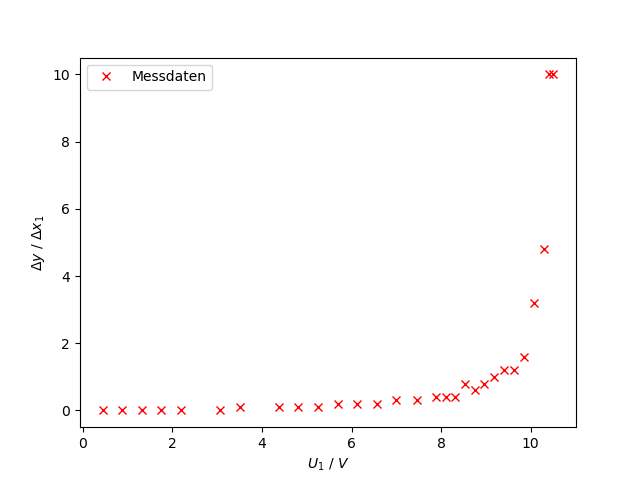
\includegraphics[height=80mm]{bilder/1.png}
    \caption{Differentielle Energieverteilung bei $297,55\,\unit{\kelvin}$.\label{Abbildung4} }
\end{figure}

\begin{figure}[H]
    \centering
    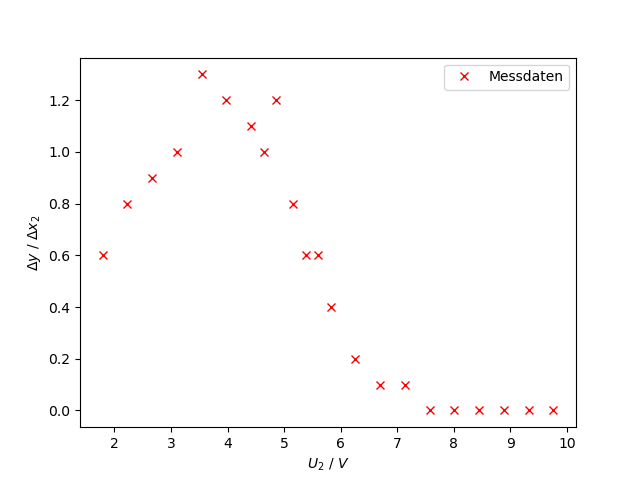
\includegraphics[height=80mm]{bilder/2.png}
    \caption{Differentielle Energieverteilung bei $422,05\,\unit{\kelvin}$.\label{Abbildung5} }
\end{figure}

\begin{flushleft}
    In der Abbildung \ref{Abbildung4} lässt sich ablesen, dass fast alle Elektronen die Energie $(10,5 \pm 0,1)\,\text{eV}$ besitzen. 
    Wird dieser Wert von der Beschleunigungsspannung $\text{U}_{\text{B}} = 11\,\unit{\volt}$ subtrahiert ergibt sich für das Kontaktpotential $\text{k} = 0,5\,\unit{\volt}$.
\end{flushleft}

\begin{flushleft}
    Aufgrund von Temperatur Fluktuationen werden die ersten sieben Messwerte nicht betrachtet. 
    Bei dem zweiten Graphen ist ein Energiemaximum nicht mehr erkenntlich, Abbildung \ref{Abbildung5}.
    Dies liegt an dem Verhältnis $\text{a} \mathbin{/} \overline{\omega}$, welches hier deutlich höher ist.
    Somit treten mehr elastische Stöße auf, welche die Richtung der Elektronen beeinflussen.
    Dies führt zu einer deutlich geringeren Zahl an Elektronen, die an der Auffängerelektrode registriert werden, so dass die Energieverteilung in Feldrichtung verwischt wird und keinen Zusammenhang zur Fermi-Dirac-Verteilung mehr zeigt.
    Nach einiger Zeit wird die Beschleunigungsspannung größer als die Spannung der Auffängerelektrode. 
    Wenn die Elektronenenergie den Wert $\text{E}_{1} - \text{E}_{0}$ erreicht, kommt es zu unelastischen Stößen und die Elektronen verlieren ihre Energie.
    Dann können sie nicht,mehr zu Auffängerelektrode gelangen.
\end{flushleft}

\begin{flushleft}
    Auffällig ist zu dem, dass bei der zweiten Messreihe kaum Elektronen mit einer Energie über ungefähr $6\,\text{eV}$ die Auffängerelektrode erreichen.
    Dabei fällt die Kurve bei ca. $4\,\text{eV}$.
    Das liegt daran, dass die im Kapitel \ref{sec:Kap1} bestimmte Anregungsenergie von Quecksilber ungefähr bei $4,9\,\text{eV}$ liegt.
\end{flushleft}

\subsection{Franck-Hertz-Kurven} \label{sec:Kap1}

\begin{flushleft}
    Mithilfe der Franck-Hertz-Kurven, siehe Kapitel \ref{sec:Anh1}, soll im Folgenden die erste Anregungsenergie für Quecksilber untersucht werden.
    Dafür werden auf dem Graphen die Abstände zwischen den Maxima gemessen.
    Die gemessenen Werte sind in der folgenden Tabelle eingetragen.
\end{flushleft}

\begin{table}[H]
    \centering
    \caption{Die Abstände zwischen den Maxima.} 
    \label{Tabelle3}
    \begin{tabular} {c  c  c  c}
        \toprule
        {$ \increment \text{x}_{\text{S}} \mathbin{/} \unit{\milli\meter} $} &
        {$ \increment \text{U}_{\text{S}} \mathbin{/} \unit{\volt} $} &
        {$ \increment \text{x}_{\text{B}} \mathbin{/} \unit{\milli\meter} $} &
        {$ \increment \text{U}_{\text{B}} \mathbin{/} \unit{\volt} $} \\
        \midrule
         29 & 4,40 & 29 & 4,40 \\
         30 & 4,56 & 29 & 4,40 \\
         31 & 4,71 & 30 & 4,56 \\
         31 & 4,71 & 31 & 4,56 \\
         31 & 4,71 & 31 & 4,71 \\
        \bottomrule
    \end{tabular} 
\end{table}

\begin{align}
    \intertext{Mit Werten aus Tabelle \ref{Tabelle3} ergibt sich, dann für die durchschnittliche Energiedifferenz folgende Werte } 
    \increment \text{E}_{\text{S}} = ( 4,62 \pm 0,12 )\,\text{eV}\,, \notag \\
    \increment \text{E}_{\text{B}} = ( 4,53 \pm 0,11 )\,\text{eV}\,. \notag
    \intertext{Gemäß der Formel \ref{3} und $\lambda = \frac{\text{c}}{\nu}$ kann aus der Energiedifferenz die Wellenlänge des emittierten Lichtes bestimmt werden }
    \lambda_{\text{B}} = \frac{\text{c}}{\nu} = \frac{\text{c}\hslash}{\increment \text{E}_{\text{B}}} = ( 273,33 \pm 0,52 )\,\unit{\nano\meter}\,, \label{7} \\
    \lambda_{\text{S}} = ( 267,99 \pm 1,60 )\,\unit{\nano\meter}\,. \notag
    \intertext{Mit der Franck-Hertz-Kurve kann erneut das Kontaktpotential bestimmt werden.
    Das erste Maximum ist um den Wert K des Kontaktpotentials verschoben.
    Da bei der gemessenen Kurve erst das zweite Maximum mit großer Sicherheit lokalisiert werden kann, gilt für das Kontaktpotential folgende Relation}
    \text{K} = \text{U}_{2} \cdot 2 \cdot (\increment \text{E})\,. \label{8}
    \intertext{Somit folgt}
    \text{K}_{\text{B}} = ( 0,64 \pm 0,08)\,, \notag \\
    \text{K}_{\text{S}} = ( 0,48 \pm 0,06)\,. \notag
\end{align}